\documentclass{article}
\usepackage{amsmath}
\usepackage{amssymb}
\usepackage{graphicx}
\usepackage{hyperref}
\usepackage[version=4]{mhchem}

\title{Problem 3}
\date{}

\begin{document}
\maketitle

\section*{Problem}
(2006 AMC 12 B) Circles with centers \(O\) and \(P\) have radii 2 and 4, respectively, and are externally tangent. Points \(A\) and \(B\) are on the circle centered at \(O\), and points \(C\) and \(D\) are on the circle centered at \(P\), such that \(A D\) and \(B C\) are common external tangents to the circles. What is the area of hexagon \(A O B C P D\) ?\\
\centering
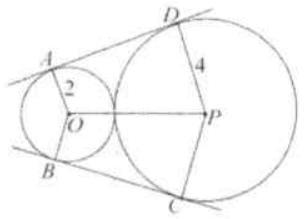
\includegraphics[width=\textwidth]{images/problem_image_1.jpg}\\
(A) \(18 \sqrt{3}\)\\
(B) \(24 \sqrt{2}\)\\
(C) 36\\
(D) \(24 \sqrt{3}\)\\
(E) \(32 \sqrt{2}\)

\section*{Solution}
(B).
Through \(O\) draw a line parallel to \(A D\) intersecting \(P D\) at \(F\). Then \(A O F D\) is a rectangle and \(O P F\) is a right triangle. Thus \(D F=2, F P=2\), and \(O F=4 \sqrt{2}\). The area of trapezoid \(A O P D\) is \(12 \sqrt{2}\), and the area of hexagon\\
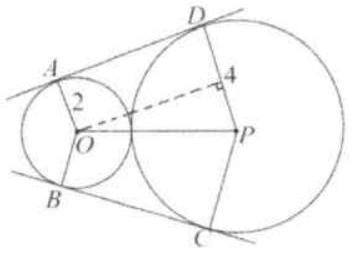
\includegraphics[width=\textwidth]{images/reasoning_image_1.jpg} \(A O B C P D\) is \(2 \times 12 \sqrt{2}=24 \sqrt{2}\).

\end{document}
